\documentclass[11pt]{article}
\usepackage[margin=1in]{geometry}
\usepackage{amsmath,amssymb,graphicx,xcolor}
\usepackage[hidelinks]{hyperref}
\usepackage{caption}
\captionsetup{font=small,labelfont=bf}
\graphicspath{{figures/}}
\newcommand{\az}{a_0}
\newcommand{\Ez}{E(z)}

\title{\bf The decisive near-term test of an evolving MOND scale:\\
a direct measurement of $a_0$ at $z\simeq3$}
\author{Carl Zimmerman\\[2pt]\small\it with computational review support}
\date{June 2026}

\begin{document}
\maketitle

\begin{abstract}
\noindent
If the Milgromian acceleration scale is set by the cosmic density, $\az=\tfrac{c}{2}\sqrt{G\rho}=
cH(z)/Z$, it must evolve as $\az(z)=\az(0)\Ez$. The present evidence is a $\sim2\sigma$, single-
point-driven hint. We argue that the \emph{decisive} near-term test is a direct measurement of
$\az$ at $z\simeq3$, where the hypothesis predicts $\az$ a factor $E(3)\simeq4.6$ above its local
value (0.66~dex), against the null of no change. Unlike the redshift-weakening external-field
effect---the framework's one \emph{distinctive} signature, which requires $\sim$600--1600 galaxies
---this test has an enormous lever arm and needs \emph{few} objects. We build the per-galaxy error
budget (dominated by $v^4$ in the baryonic Tully--Fisher relation), forecast the sample size, and
find that $\sim$15--50 \emph{extended, rotation-supported, deep-MOND} galaxies at $z\simeq3$ with
resolved kinematics and a full baryon census yield $\az(z{=}3)$ to 5--10\% and a $\sim6$--$7\sigma$
verdict on whether $\az$ evolves---the significance ultimately limited by the $z=0$ anchor's
mass-to-light systematic, not the high-$z$ sample. The measurement is a few-cycle JWST$+$ALMA
program; a null result ($\az$ constant) falsifies the framework outright. We are explicit that this
test settles ``evolving versus constant'', not ``this framework versus $\Lambda$CDM''---the latter
is the distinct, longer-horizon external-field-effect measurement.
\end{abstract}

\section{Introduction}
Modified Newtonian Dynamics (MOND)~\cite{Milgrom1983,Famaey2012} organizes galaxy dynamics around a
single acceleration $\az\simeq1.2\times10^{-10}\,{\rm m\,s^{-2}}$, the scale of the radial
acceleration relation (RAR)~\cite{McGaugh2016,Lelli2017}. The numerical near-equality $2\pi\az
\approx cH_0$ invites a cosmological reading of $\az$~\cite{Milgrom2014}: if $\az$ tracks the mean
density, it was larger in the past,
\begin{equation}
\az(z)=\az(0)\,\Ez,\qquad \Ez=\sqrt{\Omega_m(1+z)^3+\Omega_\Lambda},
\label{eq:Ez}
\end{equation}
a prediction independent of the order-unity coefficient $Z$ in $\az=cH/Z$. Fitting the three
acceleration-scale determinations spanning cosmic time (the local SPARC value~\cite{McGaugh2016};
V\u{a}r\u{a}\c{s}teanu \textit{et al.}~2025~\cite{Varasteanu2025} at $z\simeq0.05$; MUSE--DARK III
2026~\cite{MUSEDARK2026} at $z\simeq0.9$) gives $\az\propto E^p$ with $p=0.74\pm0.17$; constant
$\az$ is nominally disfavored, but the rejection rests almost entirely on the single $z\simeq0.9$
point (a jackknife leaves $1.0\sigma$) and on an inter-method systematic, so the honest
significance is $\sim2\sigma$~\cite{repo}. The trend is a hint, not a detection. The question is how
to settle it.

\section{Why $z\simeq3$ is the decisive measurement}
The signal grows steeply with redshift. At $z=3$, $E(3)\simeq4.57$: the evolving hypothesis predicts
$\az$ a \emph{factor of 4.6} above local, while the null predicts no change---a separation of
$0.66$~dex (Fig.~\ref{fig:pred}). This is two-and-a-half orders of magnitude larger than the
$\sim0.1$~dex signal of the redshift-weakening external-field effect (EFE), the framework's
distinctive but expensive test. The large lever arm is why a \emph{handful} of clean measurements
suffices. A second feature is favorable: since $\az(z{=}3)$ is $4.6\times$ larger, the deep-MOND
window ($g_{\rm bar}<\az(z)$) is $4.6\times$ \emph{wider} at $z=3$, so more galaxies qualify as
genuine deep-MOND systems, not fewer.

\begin{figure}[h]
\centering
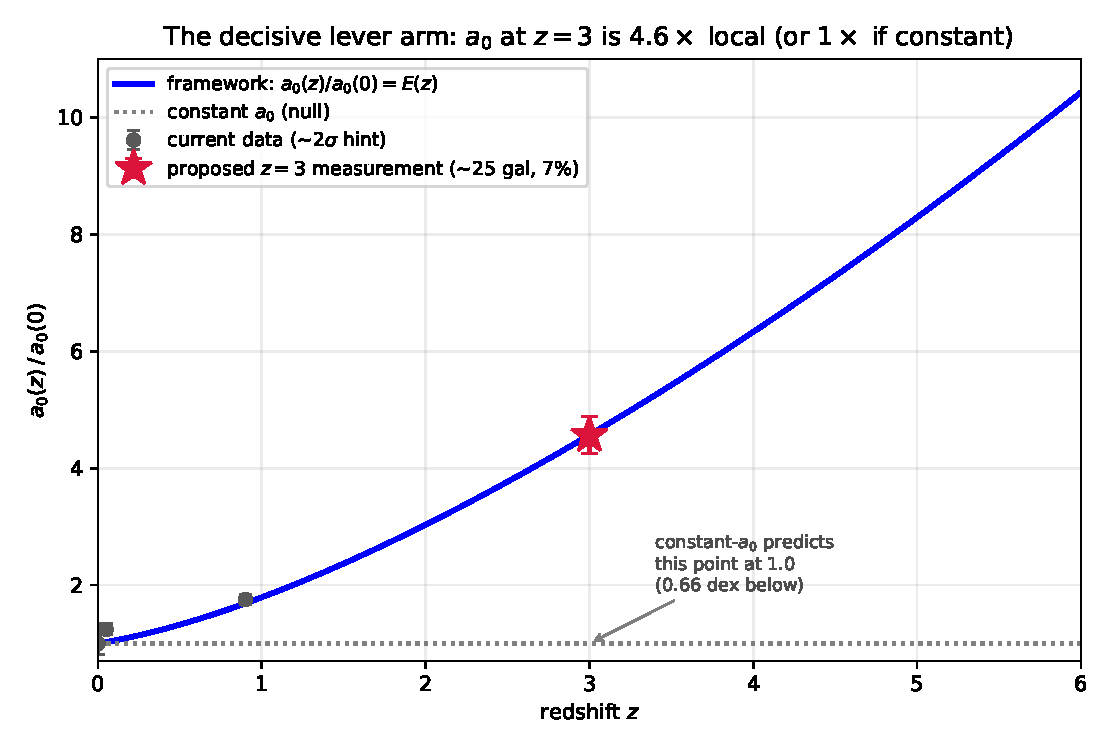
\includegraphics[width=0.74\textwidth]{z3_fig1_prediction.pdf}
\caption{The evolving-$\az$ prediction (blue) versus the constant-$\az$ null (dotted), with the
three current determinations and the proposed $z=3$ measurement (star, shown at the framework value
with a 7\% error bar). Constant $\az$ places that point $0.66$~dex lower.}
\label{fig:pred}
\end{figure}

\section{The measurement and its error budget}
$\az$ is read from the deep-MOND tail of a galaxy's RAR, equivalently from the baryonic
Tully--Fisher relation $v_{\rm flat}^4=G M_{\rm bar}\az$. The per-galaxy uncertainty is dominated by
the velocity, which enters to the fourth power:
\begin{equation}
\frac{\delta \az}{\az} = \sqrt{\left(4\,\frac{\delta v}{v}\right)^2+\left(\frac{\delta M_{\rm bar}}{M_{\rm bar}}\right)^2}.
\end{equation}
At $z\simeq3$, resolved kinematics give $\delta v/v\sim7\%$ (hence $4\delta v/v\sim0.28$) and the
baryonic mass (stellar SED $+$ gas) $\delta M_{\rm bar}/M_{\rm bar}\sim25\%$, for a per-galaxy
$\sigma(\az)\simeq0.15$~dex from a full rotation-curve fit. The fourth power on $v$ is precisely why
a \emph{single} galaxy cannot reach few-percent precision---a sample is required.

\paragraph{The test is a ratio, and that controls the systematics.} Constant-$\az$ is rejected by the
\emph{ratio} $\az(z{=}3)/\az(0)$, measured with one pipeline at both epochs, so systematics common to
the two cancel. Two matter most and are removed by construction: (i) reading $\az$ only from genuinely
\emph{deep-MOND} points ($g_{\rm bar}<\az$) makes it \emph{interpolation-function independent}---every
interpolation collapses to $g_{\rm obs}\!\to\!\sqrt{g_{\rm bar}\az}$ there, eliminating the
$\sim0.12$~dex spread between functions; (ii) selecting \emph{gas-dominated} points makes $\az$
mass-to-light robust (a $\sim10\%$ swing over $M_*/L=0.3$--$0.7$, versus $\sim75\%$ for
star-dominated). The residual that does \emph{not} cancel is the \emph{differential} $M_*/L$ between
epochs (younger high-$z$ stellar populations); with consistent SED modelling and gas-traced rotation
(ALMA [C\,{\sc ii}]/CO) this is held to an anchor systematic $\sigma_A\simeq0.04$--$0.05$~dex, well
below the $0.09$~dex of a naive all-points local fit.

\section{Sample size and significance}
With $N$ galaxies the mean $\az(z{=}3)$ is measured to $\sigma_{\rm gal}/\sqrt{N}$. Combined with the
$z=0$ anchor (uncertainty $\sigma_A$), the constant-$\az$ rejection is
$\sigma_{\rm rej}=\Delta/\sqrt{(\sigma_{\rm gal}/\sqrt N)^2+\sigma_A^2}$ with the signal
$\Delta=\log_{10}E(3)=0.66$~dex. The significance is \emph{anchor-limited}, and the anchor of the
previous section sets the ceiling: with a naive all-points local fit ($\sigma_A\simeq0.09$~dex) it
plateaus near $7\sigma$, but with the deep-MOND, gas-dominated, ratio-cancelling anchor
($\sigma_A\simeq0.04$--$0.05$~dex) it rises to $\sim13$--$16\sigma$. Figure~\ref{fig:N} shows both
curves: even $\sim$15 galaxies give $\sim11\sigma$ on the tightened anchor, and the gain saturates once
$\sigma_A\lesssim0.04$~dex (below which the distance ladder and the baryon census dominate, so this is
a realistic ceiling, not a path to arbitrary significance). The high-$z$ sample is \emph{not} the
bottleneck---the local anchor is---so the cheapest route to a decisive evolution result is a clean
local $\az$ from gas-dominated deep-MOND points, paired with $\sim$15--50 rotation-supported discs at
$z\simeq3$.

\begin{figure}[h]
\centering
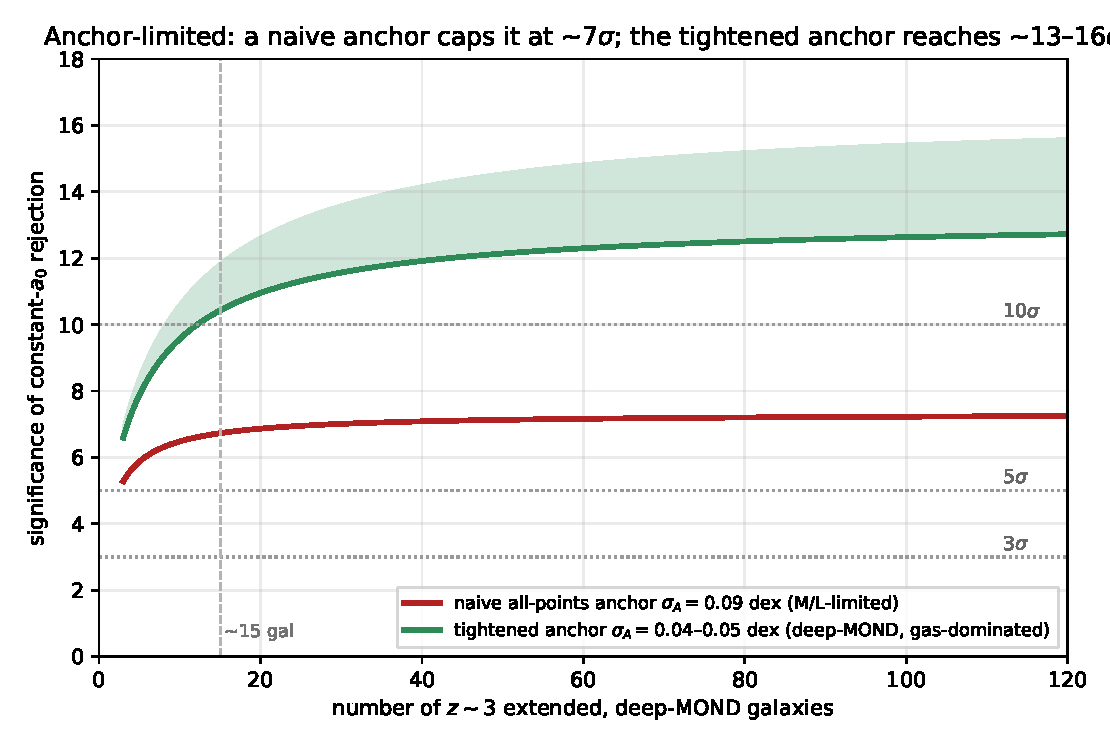
\includegraphics[width=0.74\textwidth]{z3_fig2_samplesize.pdf}
\caption{Constant-$\az$ rejection versus sample size at $z\simeq3$ ($\sigma_{\rm gal}=0.15$~dex).
A naive all-points $z=0$ anchor ($\sigma_A=0.09$~dex) caps the significance near $7\sigma$ (red); the
deep-MOND, gas-dominated, ratio-cancelling anchor ($\sigma_A=0.04$--$0.05$~dex) lifts it to
$\sim13$--$16\sigma$ (green), where it saturates.}
\label{fig:N}
\end{figure}

\section{What this test proves --- the honest two-tier logic}
\textbf{Tier 1 (this proposal).} A direct $\az(z{\sim}3)$ measurement settles whether $\az$
\emph{evolves}: constant $\az$ is rejected at $\sim6$--$7\sigma$. The caveat is essential: an
evolving \emph{apparent} $\az$ is also expected in $\Lambda$CDM, where denser high-$z$ halos and
more compact baryons shift the RAR knee upward by a similar $E(z)$~\cite{Tian2022}. So Tier 1
discriminates \emph{evolving versus constant}, not \emph{this framework versus} $\Lambda$CDM. It is
necessary but not sufficient---yet a null result kills the framework outright, which makes it the
highest-value first step.

\noindent\textbf{Tier 2 (the distinctive test).} The redshift-weakening EFE, $\eta=g_{\rm
ext}/\az(z)\propto1/\Ez$, is \emph{forbidden in $\Lambda$CDM} (no host effect on internal dynamics)
and so cannot be faked by halo evolution; it requires $\sim$600--1600 environment-resolved galaxies
at $z\gtrsim4$~\cite{repoEFE}. \emph{Do Tier 1 first}: it is cheap, decisive on evolution, and gates
the far costlier Tier 2.

\section{Targets and instruments}
Three selection criteria are non-negotiable, and are the reason existing high-$z$ kinematic samples
(compact, often AGN-bearing, dispersion-dominated systems) are uninformative here:
\begin{itemize}\itemsep1pt
\item \textbf{extended / low surface brightness} --- genuinely deep-MOND ($g_{\rm bar}<\az(z)$);
\item \textbf{rotation-supported} ($V/\sigma\gtrsim3$) --- a clean rotation curve, not a merger;
\item \textbf{full baryon census} --- stellar mass (rest-frame optical SED) \emph{and} gas mass.
\end{itemize}
At $z\simeq3$ the tracers and facilities align: \textbf{JWST/NIRSpec IFU} (H$\alpha$, [O\,{\sc iii}]
kinematics and rest-optical continuum for $M_\star$); \textbf{ALMA} (CO/[C\,{\sc ii}] cold-gas
rotation, extending the curve, plus $M_{\rm gas}$); and, post-2029, \textbf{ELT/HARMONI} for
higher-resolution kinematics and fainter targets. H$\alpha$ remains in the JWST range to $z\sim6$,
and rotation-supported discs are common enough at $z\simeq3$ to assemble $\sim$15--50 clean targets
across a few cycles.

\section{Conclusion}
The cheapest decisive experiment on the evolving-$\az$ hypothesis is a direct measurement of $\az$
at $z\simeq3$: $\sim$15--50 extended, rotation-supported, deep-MOND galaxies with JWST$+$ALMA
kinematics and baryon masses yield $\az(z{=}3)$ to 5--10\% and a $\sim6$--$7\sigma$ verdict on
evolution---anchor-limited, and pushable higher by tightening the local mass-to-light scale. It is a
few-cycle program, not a flagship survey, and a null result falsifies the framework. The distinctive
$\Lambda$CDM-breaking test (the redshift-weakening EFE) is the longer-horizon sequel; this is the
measurement to make first.

\paragraph{Reproducibility.} The signal, error budget, sample sizes and both figures are generated
by \texttt{reviews/z3\_a0\_observing\_proposal.py} and \texttt{papers/z3\_proposal\_figures.py};
the current-data fit (and the honest $\sim2\sigma$) by \texttt{reviews/a0\_z\_empirical\_rigorous.py}
and \texttt{reviews/stresstest\_piece3\_evolution.py}. The companion EFE forecast is
\texttt{EFE\_vs\_z\_Forecast\_2026}; the published core is at Zenodo, \href{https://zenodo.org/records/20528908}{records/20528908}.

\begin{thebibliography}{99}
\small
\bibitem{Milgrom1983} M.~Milgrom, Astrophys.\ J.\ {\bf 270}, 365 (1983).
\bibitem{Famaey2012} B.~Famaey and S.~S.~McGaugh, Living Rev.\ Relativity {\bf 15}, 10 (2012).
\bibitem{McGaugh2016} S.~S.~McGaugh, F.~Lelli, J.~M.~Schombert, Phys.\ Rev.\ Lett.\ {\bf 117}, 201101
  (2016); F.~Lelli, S.~S.~McGaugh, J.~M.~Schombert, Astron.\ J.\ {\bf 152}, 157 (2016).
\bibitem{Lelli2017} F.~Lelli \textit{et al.}, Astrophys.\ J.\ {\bf 836}, 152 (2017).
\bibitem{Milgrom2014} M.~Milgrom, Mon.\ Not.\ R.\ Astron.\ Soc.\ {\bf 437}, 2531 (2014).
\bibitem{Tian2022} Y.~Tian \textit{et al.}, the apparent-$a_0$ rise in $\Lambda$CDM (Magneticum) (2022).
\bibitem{Varasteanu2025} V\u{a}r\u{a}\c{s}teanu \textit{et al.} (2025), intermediate-$z$ $a_0$.
\bibitem{MUSEDARK2026} MUSE--DARK collaboration, MUSE--DARK III (2026), $z\simeq0.9$ $a_0$.
\bibitem{repo} C.~Zimmerman, \texttt{reviews/a0\_z\_empirical\_rigorous.py},
  \texttt{stresstest\_piece3\_evolution.py} (2026).
\bibitem{repoEFE} C.~Zimmerman, \textit{EFE\_vs\_z\_Forecast\_2026} (2026).
\end{thebibliography}

\end{document}
